\section{Results}
\label{sec:results}

\subsection{Short references and their fix}
The first-30 reference had a condition number above $10^{10}$ in all 62 sessions (median about $3 \times 10^{14}$), against about $5 \times 10^{3}$ for whole-session references in the median. The pre-processed EEG is rank-deficient, and the null directions appear to change over a session, so a short average leaves near-zero eigenvalues that amplify later signal. Accuracy collapsed accordingly (Table~\ref{tab:main}; AUC 0.533). Shrinkage at $\alpha = 0.1$ brought the condition number to about 150 and restored accuracy to 74.79\%.

\begin{table}[!t]
\centering
\caption{Online Alignment on 27 Subjects, Five Seeds. Trials from the 31st of Each Session; $\Delta$ and $p$ Against No Alignment}
\label{tab:main}
\footnotesize
\setlength{\tabcolsep}{3pt}
\begin{tabularx}{\columnwidth}{@{}YL{0.8cm}L{0.8cm}L{0.75cm}L{0.8cm}L{0.8cm}@{}}
\toprule
\textbf{Method} & \textbf{Bal. acc.} & \textbf{$\Delta$} & \textbf{W/L} & \textbf{$p$} & \textbf{AUC} \\
\midrule
No alignment & 73.59 & -- & -- & -- & 0.828 \\
\midrule
\multicolumn{6}{@{}l}{\textit{No regularisation}} \\
First 30 & 52.55 & $-21.04$ & 3/24 & $<$0.001 & 0.533 \\
Cumulative & 75.26 & $+1.67$ & 13/14 & 0.66 & 0.802 \\
Last 100 & 71.76 & $-1.83$ & 8/19 & 0.17 & 0.765 \\
Whole session & 77.85 & $+4.26$ & 19/8 & 0.019 & 0.834 \\
\midrule
\multicolumn{6}{@{}l}{\textit{Shrinkage, $\alpha = 0.1$}} \\
First 30 & 74.79 & $+1.20$ & 14/13 & 0.55 & 0.801 \\
Cumulative & 76.25 & $+2.66$ & 16/11 & 0.155 & 0.818 \\
Last 100 & 74.77 & $+1.18$ & 12/15 & 0.86 & 0.810 \\
Whole session & 77.27 & $+3.68$ & 18/9 & 0.032 & 0.832 \\
\midrule
\multicolumn{6}{@{}l}{\textit{Population prior}} \\
$\kappa = 30$ (primary) & 77.37 & $+3.78$ & 18/9 & 0.039 & 0.820 \\
$\kappa = 10$ & 77.01 & $+3.42$ & 17/10 & 0.065 & 0.817 \\
$\kappa = 100$ & 77.08 & $+3.49$ & 18/9 & 0.032 & 0.820 \\
$R_{\mathrm{pop}}$ only & 74.12 & $+0.53$ & 13/14 & 0.75 & 0.804 \\
\bottomrule
\end{tabularx}
\end{table}

\subsection{Online alignment}
The prespecified test favoured the prior: $+3.78$ points against no alignment (18/9 subjects, $p = 0.039$). It showed no detectable loss against whole-session alignment without shrinkage ($-0.48$, $p = 0.90$). The result is sensitive to a few drivers: the median gain is 2.41 points, and removing the subject with the largest gain (34.3 points) gives $+2.60$ ($p = 0.067$). AUC did not improve ($-0.009$, $p = 0.46$), so the gain looks like better threshold calibration for a new driver, not better ranking; whole-session alignment shows the same pattern. The prior was not significantly better than shrunk cumulative alignment ($+1.11$, $p = 0.20$). The prior alone gave no gain, and the full method beat it ($+3.25$, 20/7, $p = 0.013$, not prespecified), so the benefit comes from the driver's own data.

\subsection{Time course}
Fig.~\ref{fig:time} shows when the gain arrives. It is absent early: the prior gains $+0.18$ points in trials 31--100, and $-3.72$ on the first 30 trials (10 subjects, $p = 0.13$), so the prior prevents instability but does not bring an early benefit. Gains appear in the middle of the session ($+5.96$ in trials 201--300, 13/5, $p = 0.0096$). A frozen first-30 reference loses 6.40 points after trial 300 (2/13, $p = 0.0015$). Across all scored trials, the running prior beat the frozen reference by 2.57 points (18/9, $p = 0.08$), although the two used different training regularisation. These bins are exploratory and contain different subjects.

\begin{figure}[!t]
\centering
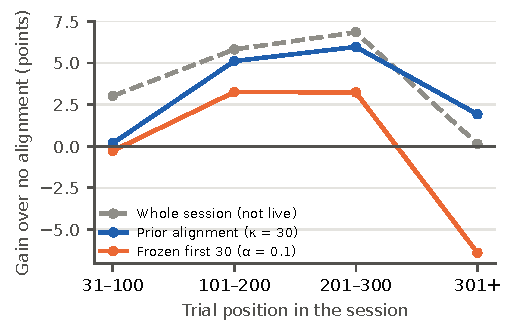
\includegraphics[width=\columnwidth]{fig2_time}
\caption{Gain over no alignment by trial position, five seeds. Each point compares subjects with both classes in that bin; subject sets differ between bins. Exploratory.}
\label{fig:time}
\end{figure}

\subsection{State mix}
Fig.~\ref{fig:statemix} shows the gain by drowsy share so far. For the prior it was $+1.22$ and $+1.24$ points below 25\%, $+7.70$ at 25--50\% (12/4, $p = 0.0076$), $+12.47$ at 50--75\% (8/3, $p = 0.032$) and $+1.18$ above 75\% (2/4, 6 subjects, $p = 1.0$). Shrunk cumulative alignment has the same shape. This resembles our earlier inverted U on the 11-subject subset, where windows were built with fixed mixes, so the pattern appears both with constructed references and on real timelines. Two limits apply. These tests are uncorrected, and the upper bins contain few subjects. More importantly, drowsy share rises with time on task, so we cannot separate state mix from elapsed time here. \todo{Consider the within-time-bin check before submitting.}

\begin{figure}[!t]
\centering
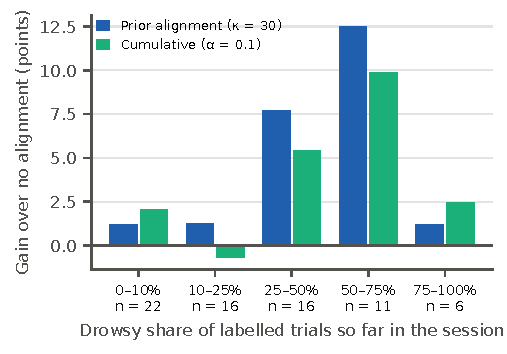
\includegraphics[width=\columnwidth]{fig1_statemix}
\caption{Gain over no alignment by drowsy share of labelled trials so far in the session; $n$ is the number of subjects with both classes in that bin. Exploratory and entangled with time on task.}
\label{fig:statemix}
\end{figure}

\subsection{Batch-norm adaptation}
Table~\ref{tab:bn} shows that updating batch-norm statistics hurt in every setting. The prespecified comparison favoured prior alignment over blended adaptation by 6.81 points (23/4, $p = 0.0008$; AUC difference not significant, $p = 0.19$). Adding the update to prior alignment was worse: at the setting of Duan \textit{et al.}, accuracy fell to 53.84\% (2/25, $p < 0.0001$). The harm grew as the statistics gave more weight to the current window. This model decides from the time-averaged output of its batch-norm layer, so statistics dominated by the current window subtract much of the evidence; we reasoned this from the architecture and did not test it separately. With Riemannian logistic regression, the prior gave no gain ($-0.17$, $p = 0.99$) and AUC fell from 0.739 to 0.701, so the alignment benefit is not model-independent either.

\begin{table}[!t]
\centering
\caption{Batch-Norm Adaptation, Five Seeds. $\Delta$ Against No Alignment (73.59\%)}
\label{tab:bn}
\footnotesize
\setlength{\tabcolsep}{3pt}
\begin{tabularx}{\columnwidth}{@{}YL{0.8cm}L{0.85cm}L{0.7cm}L{0.8cm}@{}}
\toprule
\textbf{Method} & \textbf{Bal. acc.} & \textbf{$\Delta$} & \textbf{W/L} & \textbf{AUC} \\
\midrule
\multicolumn{5}{@{}l}{\textit{Without alignment}} \\
Blend, weight 100 & 71.05 & $-2.54$ & 8/19 & 0.815 \\
Blend, weight 30 & 70.56 & $-3.03$ & 8/19 & 0.802 \\
Blend, weight 10 & 70.09 & $-3.50$ & 9/18 & 0.794 \\
Moving average, 0.1 & 59.58 & $-14.01$ & 3/24 & 0.651 \\
\midrule
\multicolumn{5}{@{}l}{\textit{With prior alignment (77.37\% alone)}} \\
Blend, weight 30 & 70.76 & $-2.83$ & -- & 0.774 \\
Moving average, 0.1 & 59.88 & $-13.71$ & -- & 0.640 \\
Moving average, 0.7 & 53.84 & $-19.75$ & -- & 0.551 \\
\bottomrule
\end{tabularx}
\end{table}

\subsection{Explanations under alignment}
Table~\ref{tab:xai} gives the prespecified removal tests. Alignment increased the model's reliance on gamma for alert decisions and on theta for drowsy decisions; alpha and central-channel effects did not differ. Theta is an established drowsiness marker, whereas gamma overlaps muscle activity, so the gamma shift may be a shortcut, although this test does not establish that. The peripheral result needs caution: zeroing 15 channels under a fixed whitener disturbs its channel mixing, and relevance maps point the other way, with the peripheral share falling from 54\% to 36\% for gradient$\times$input.

Attributions weakened. Under alignment, gradient$\times$input still beat random point deletion on all 27 subjects, but with a narrower margin (area 0.635 against 0.671 for random; without alignment 0.511 against 0.789). Correlation with maps from a randomised model rose from 0.117 to 0.366 for saliency and from 0.503 to 0.599 for gradient$\times$input, as a fixed whitener shapes the maps whatever the weights are.

\begin{table}[!t]
\centering
\caption{Change in P(True Class) When Removing a Band or Channel Group. Prespecified, Holm-Corrected Over Six Tests}
\label{tab:xai}
\footnotesize
\setlength{\tabcolsep}{3pt}
\begin{tabularx}{\columnwidth}{@{}YL{1cm}L{1cm}L{1.25cm}@{}}
\toprule
\textbf{Removed; class} & \textbf{None} & \textbf{Prior} & \textbf{Holm $p$} \\
\midrule
Gamma; alert & $-0.074$ & $-0.195$ & $<$0.001 \\
Beta; alert & $+0.054$ & $+0.074$ & 0.003 \\
Peripheral; alert & $-0.110$ & $+0.207$ & $<$0.001 \\
Theta; drowsy & $-0.244$ & $-0.300$ & $<$0.001 \\
Alpha; drowsy & $-0.070$ & $-0.061$ & 0.57 \\
Central; drowsy & $-0.361$ & $-0.402$ & 0.57 \\
\bottomrule
\end{tabularx}
\end{table}

\subsection{Computational cost}
On a Kaggle CPU with one window at a time, the whitening update took a median of 0.85 ms and a forward pass 0.59 ms, so the computation is cheap enough for live use. We did not test on in-vehicle hardware.
